\section{Package Location}

\indent Figure \ref{fig:PackageLocation} is an Abaqus visualization of the Newport Bridge with the proposed location for the sensor package to be mounted.
As shown in the figure, the center of the bridge is the best location for the sensor package. This is because the greatest amplitude of displacement will
occur during the first mode of vibration at the middle of the bridge. Mounting the sensor package to the bridge must be done without damaging the
structure in any way. The sensor package must also be capable of being moved easily. Most importantly, the package must be secured without any of its
own motion so that the sensors can recognize the movement of the bridge and not the movement of the package itself. 

The most economical way of securing the sensor package to the bridge is to use powerful magnets. Neodymium Magnets are strong magnets that work well in
all environments and resist demagnetization. One negative aspect of magnets is that they can be prone to corrosion if a protective coating is not
properly applied. There is also a concern that the magnetic field can disrupt the electronics within the case. However, these issues can be prevented if
the correct precautions are taken. These magnets come in many shapes and sizes, as shown in Figure \ref{fig:Mounting Magnet}, and can be purchased with
pre-fabricated holes for screws to attach the magnets to the exterior of the case. The magnets in figure \ref{fig:Mounting Magnet} are the MMR-A-XC
model of magnets from KJMagnetics.com. This magnet is hardly larger than a penny, yet it can easily be screwed into the sensor package and has a
holding force of 54.14 pounds. With two of these magnets screwed into the case, the package would be secured to the bridge. If data analysis is
performed to prove the wind speed on the surface of the package to be too much for this pull force, stronger magnets are available. KJMagnetics.com
also has similar magnets but with different pull forces ranging from 26.8 pounds to 260 pounds. These magnets can be used for securing the solar
panels and wind turbine as well. 

\begin{figure}[ht]
\centering
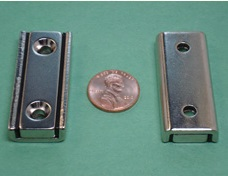
\includegraphics[width=0.5\textwidth]{Neodymium_Mounting_Magnet.jpg}
\caption{Neodymium Mounting Magnet.}
\label{fig:Mounting Magnet}
\end{figure}

Figure \ref{fig:Proposed Package, Panels and Turbine Location} shows a practicable location for the sensor package along with the solar panels above and
the wind turbine hanging just below. The sensor package should be mounted on the outside of one of the major vertical beams at midspan of the bridge. The
solar panels and wind turbine must be mounted close within a reasonable distance to keep the cable length to a minimum. The best place to mount the
solar panels is on top of the upper horizontal beam on the southern side of the bridge. This will allow for the most amount of sun light and the
shortest amount of cable necessary. The best place to mount the wind turbine is on the bottom of the lower horizontal beam on the southern side of the
bridge. This location has plenty of wind because it is above the middle of the Narragansett Bay. By mounting the sensor package, solar panels and
wind turbine below the deck on the southern side of the bridge the package will be capable of producing its own power and accurately measuring the
vibrations of the bridge.


\begin{figure}[ht]
\centering
\includegraphics[width=\textwidth]{Bridge_Full_.png}
\caption{Proposed Package Mounting Location.}
\label{fig:PackageLocation}
\end{figure}


\begin{figure}[ht]
\centering
\includegraphics[width=0.75\textwidth]{Proposed_Package_Location.png}
\caption{Proposed Location for Sensor Package, Wind Turbine and Solar Panels.}
\label{fig:Proposed Package, Panels and Turbine Location}
\end{figure}
